\documentclass [article, 12pt, a4paper, oneside, section=TITLE]{abntex2}


\usepackage[utf8]{inputenc}
\usepackage[T1]{fontenc}
\usepackage[english, main=brazil]{babel}
\usepackage{amsmath}
\usepackage{amssymb,amsfonts,textcomp}
\usepackage{color}
\usepackage{array}
\usepackage{supertabular}
\usepackage{listings}         % Para as linguagens de programação
\usepackage{lastpage}		  % Usado pela Ficha catalográfica
\usepackage{indentfirst}	  % Indenta o primeiro parágrafo de cada seção.
\usepackage{hhline}
\usepackage{hyperref}
\usepackage[pdftex]{graphicx}
\graphicspath{ {./figuras/} }


% retira as mensagens de aviso do pacote Glossaries
\let\printglossary\relax
\let\theglossary\relax
\let\endtheglossary\relax
% coloca Seções em maiúsculas sem negrito no Sumário
\makeatletter
\let\oldcontentsline\contentsline
\def\contentsline#1#2{%
  \expandafter\ifx\csname l@#1\endcsname\l@section
    \expandafter\@firstoftwo
  \else
    \expandafter\@secondoftwo
  \fi
  {%
    \oldcontentsline{#1}{\normalfont\MakeTextUppercase{#2}}%
  }{%
    \oldcontentsline{#1}{#2}%
  }%
}
\makeatother
% ---
% Pacotes glossaries
% ---
\usepackage[subentrycounter,seeautonumberlist,nonumberlist=true]{glossaries}
% para usar o xindy ao invés do makeindex:
%\usepackage[xindy={language=portuguese},subentrycounter,seeautonumberlist,nonumberlist=true]{glossaries}
% ---
% Citações de referências no formato alfabético e negrito
\usepackage[alf, abnt-emphasize=bf]{abntex2cite} 
% Margens definidas em 25 mm para uso como documento em PDF
% Para imprimir use as seguintes margens:
% \usepackage[left=30mm, top=30mm, right=20 mm, bottom=20mm] {geometry}

\usepackage[margin=25 mm]{geometry}
%---
% O arquivo com o nome dos alunos e dos orientadores é lido aqui.
% Atualizar diretamente no arquivo
%---

%%%%%%%%%%%%%%%%%%%%%%%%%%%%%%%%%%%%%%%%%%%%%%%%%%%%%%%%%%%
% Corrige a fonte dos capítulos, seções, resumos, etc.
%%%%%%%%%%%%%%%%%%%%%%%%%%%%%%%%%%%%%%%%%%%%%%%%%%%%%%%%%%%

\renewcommand{\ABNTEXchapterfont}{\bfseries \rmfamily}  % Capítulos em Bold e Maiúsculas
\renewcommand{\ABNTEXchapterfontsize}{\normalsize}
\renewcommand{\ABNTEXsectionfont}{\rmfamily}            %  Seções em  Maiúsculas apenas
\renewcommand{\ABNTEXsectionfontsize}{\normalsize}
\renewcommand{\ABNTEXsubsectionfont}{\bfseries}         % Subseções em Bold apenas
\renewcommand{\ABNTEXsubsectionfontsize}{\normalsize}
\renewcommand{\lstlistingname}{Código}                  % Nome para os códigos no texto
\renewcommand{\lstlistlistingname}{Lista de \lstlistingname s}
\makeatletter                                          % Configura a linha da lista de códigos
\renewcommand\l@lstlisting[2]{{\normalfont\@dottedtocline{1}{1.5em}{2em}{Código~#1}{#2}}}
\makeatother
\usepackage{url16023}  % para retirar < e > da URL nas referências.

\begin{document}

%===================================CAPA====================================

\thispagestyle{empty}
    \begin{center}
        
\includegraphics[scale=0.25]{imagem/ifsp-ctd.png}
        
        \Large \textbf{Instituto Federal São Paulo - Campus Catanduva}\\
        \large \textbf{IFSP - Catanduva}
        \vspace{4.5 cm}
        
        \Large \textbf{Daniel Gonçalves}\\
        \Large \textbf{Murilo dos Reis Tavares}\\
    \end{center}

    \begin{center}
        \vspace{7 cm}
        Catanduva, São Paulo \\
        2024
    \end{center}

%=============================CONTRACAPA====================================

\newpage
\thispagestyle{empty}
    %\begin{titlepage}
        \begin{center}
            \Large \textbf{Daniel Gonçalves}\\
            \Large \textbf{Murilo dos Reis Tavares}

            \vspace{3 cm}
            \Large \textbf{Comando e Monitoramento de Unidades de Escoamento ou Alimentação de Contêineres}
            
        \end{center}

        \vspace{3 cm}
        \hfill \parbox {8 cm} {Trabalho de conclusão de curso apresentado ao
        Instituto Federal São Paulo - Campus Catanduva, como parte das exigências para obtenção do título de pós-graduação em Internet das Coisas}
        \vspace{4 cm}

        \begin{table}[htb!]
            \centering
            \begin{tabular}{c|c}
                 Orientador: &
                 Coorientador: \\
                 Prof. Dr. Marcos Rodrigues Costa & 
                 Prof. Me. Edivaldo Pastori Valentini
            \end{tabular}
        \end{table}

        \begin{center}
            \vspace{5 cm}
            Catanduva, São Paulo \\
            2024
        \end{center}      
    %\end{titlepage}

%=============================DEDICATÓRIA===================================

\newpage
\thispagestyle{empty}
\begin{dedicatoria}
\vspace*{\fill}
Dedicamos este trabalho a todos que, de alguma forma, estiveram presentes em nossa jornada, contribuindo para a realização deste sonho.

\vspace{5mm}

Aos nossos familiares, pelo amor, apoio incondicional e pela confiança em nosso potencial, mesmo nos momentos de dificuldade. Às nossas famílias, por sempre estarem ao nosso lado, oferecendo o suporte necessário para que pudéssemos seguir em frente.

\vspace{5mm}

Aos nossos amigos, que, com palavras de incentivo, alegria e companheirismo, tornaram essa caminhada mais leve e cheia de significado.

\vspace{5mm}

Aos professores, por compartilharem seus conhecimentos e orientações valiosas, e por acreditarem em nosso desenvolvimento acadêmico.

\vspace{5mm}

Este trabalho é um reflexo de um esforço coletivo, e somos imensamente gratos a todos que fizeram parte dessa conquista.
\vspace*{\fill}
\end{dedicatoria}

%==============================RESUMO=======================================

\newpage
\thispagestyle{empty}
\begin{resumo}
\begin{SingleSpace}
Este trabalho implementa uma solução para medição do nível de fluidos em contêineres para monitoramento, com capacidade para reagir aos dados coletados, comandando de forma automatizada, o escoamento ou completamento do conteúdo. Dessa forma, o domínio deste trabalho está relacionado ao monitoramento de contêineres cujo conteúdo precise ser completado para manter um nível mínimo ou que precise ser escoado para evitar que ultrapasse um nível máximo. As soluções para problemas similares que encontramos utilizam uma abordagem monolítica, fazendo com que as partes responsáveis pela medição, monitoramento e escoamento ou completamento formem um único bloco indissociável. Neste projeto usamos o conceito de separar e especializar as partes, de modo que elas possam estar fisicamente distantes entre si e, ainda assim, cumprirem suas funções e se comunicarem através da infraestrutura de internet disponível, se houver. Como resultado, conseguimos validar a proposta de separar as partes da solução em unidades independentes e capazes através de microcontroladores NodeMCU, baseados no ESP32, além de outros componentes, como sensores e atuadores, bastante simples e amplamente disponíveis. Embora a Expressif Systems, fabricante das plataformas ESP32 utilizadas, indique seu uso para ambientes industriais, os demais os componentes utilizados na implementação tem um propósito muito mais didático, e podem não ser recomendados para uso em produção, principalmente em ambientes com condições agressivas de umidade e temperatura. Entretanto, foi possível verificar a viabilidade da solução, principalmente na integração com soluções de software amplamente utilizadas na indústria, como servidores de bancos de dados e de enfileiramento de mensagens para telemetria.

\end{SingleSpace}
\vspace{\onelineskip}
\textbf{Palavras-chave}: IoT, Internet das Coisas, ESP32, Monitoramento, Bomba D'água, JT100, HC-SR04, Fluído, Contêiner, WiFi, Docker, Node-RED, MQTT, Mosquitto MQTT Broker
\end{resumo}

%============================ABSTRACT=======================================

\newpage
\thispagestyle{empty}
\begin{resumo}[Abstract]
\begin{otherlanguage*}{english}
\begin{SingleSpace}
This work implements a solution for measuring fluid levels in containers for monitoring purposes, with the ability to react to the collected data by automatically controlling the draining or filling of the contents. Thus, the scope of this work is related to monitoring containers that need to be filled to maintain a minimum level or that need to be drained to avoid exceeding a maximum level. The solutions for similar problems that we encountered use a monolithic approach, causing the parts responsible for measurement, monitoring, and draining or filling to form a single, inseparable block. In this project, we use the concept of separating and specializing the parts, so they can be physically distant from each other while still fulfilling their functions and communicating through the available internet infrastructure, if any. As a result, we were able to validate the proposal of separating the solution into independent and capable units through NodeMCU microcontrollers based on the ESP32, along with other components such as sensors and actuators that are quite simple and widely available. Although Expressif Systems, the manufacturer of the ESP32 platforms used, indicates their use for industrial environments, the other components utilized in the implementation have a much more educational purpose and may not be recommended for production use, especially in environments with aggressive humidity and temperature conditions. Nevertheless, it was possible to verify the feasibility of the solution, particularly in its integration with widely used software solutions in the industry, such as database servers and message queuing systems for telemetry.
\end{SingleSpace}

\vspace{\onelineskip}
   \textbf{Keywords}: IoT, Internet of Things, ESP32, Monitoring, Water Pump, JT100, HC-SR04, Fluid, Container, WiFi, Docker, Node-RED, MQTT, Mosquitto MQTT Broker
 \end{otherlanguage*}
\end{resumo}

%=============================SUMÁRIO=======================================

\newpage
\pdfbookmark[0]{\contentsname}{toc}
\tableofcontents*
\vspace{5mm}
\listoffigures
\cleardoublepage

%=============================ELEMENTOS TEXTUAIS============================
\newpage
\pagestyle{plain}
\pagenumbering{arabic}
%\textual

\section{Introdução}

A Internet das Coisas é reconhecida como uma das mais importantes áreas de tecnologia futura e vem obtendo muita atenção de uma grande parte das indústrias \cite{lee2015internet}. Também chamada de Internet de Tudo ou Internet Industrial, trata-se de um paradigma tecnológico imaginado como uma rede global de máquinas e dispositivos capazes de interagirem entre si \cite{lee2015internet} de forma automática e sem nenhuma ou praticamente nenhuma interação humana \cite{li2006state}.

Com o objetivo de eliminar vazamentos nos reservatórios de fluidos e reduzir o desperdício gerado por esses vazamentos, a implementação de dispositivos que monitoram o consumo e os níveis de fluidos tornou-se uma solução fundamental, contribuindo tanto para a diminuição do desperdício quanto para a preservação desses recursos \cite{gurgel2021sistema}.

A medição de níveis de líquidos ou fluidos é uma demanda comum na indústria e até mesmo em residências \cite{gonccalves2019controle}, embora a natureza distribuída aqui proposta seja a possibilidade de alta escalabilidade, muito mais condizente com as necessidades da indústria \cite{tairaprototipagem}.

Portanto, foi desenvolvido um protótipo criando uma rede de unidades de dispositivos, com responsabilidades bem definidas, capazes de monitorar, mensurar e comandar o escoamento de contêineres de fluidos de qualquer natureza de forma automática e distribuída, com capacidade de escalar para qualquer número de contêineres monitorados e que possam estar exatamente ao lado um do outro ou muito distantes, a depender da infraestrutura de comunicação em uso.

\subsection{Objetivo}
O objetivo é implementar unidades distintas, utilizando componentes comuns, amplamente disponíveis e acessíveis, utilizando uma infraestrutura moderna de software e plataformas de código aberto que viabilizem a interação entre as unidades, considerando que possam ser adicionados um número virtualmente ilimitado de pares de unidades de medição e escoamento.

\subsubsection{Objetivos Específicos}
\begin{itemize}
    \item Avaliar as dificuldades de comunicação entre dispositivos capazes de publicar e receber dados de mensagens de telemetria, MQTT e de registro das medições (\textit{logging}).
    \item Arquitetar uma solução de alta coesão e baixo acoplamento permitindo a expansão da solução para um número virtualmente ilimitado de pares de unidades de medição e escoamento.

\end{itemize}

% ===== Fundamentação Teórica =====
\newpage
\section{Fundamentação Teórica}
Neste capítulo será apresentado uma introdução sobre cada uma das partes, tecnologias e componentes, mais relevantes que possibilitaram o desenvolvimento deste projeto.

\subsection{IoT}
A Internet das Coisas (IoT, do inglês Internet of Things) surgiu a partir dos avanços em diversas áreas, como sistemas embarcados, microeletrônica, comunicação e tecnologias de sensoriamento. Ela tem atraído crescente atenção no setor industrial, devido ao seu grande potencial de aplicação em uma vasta gama de atividades humanas, sendo cada vez mais reconhecida por suas possibilidades de transformação em múltiplos setores. Em resumo, a IoT pode ser vista como uma extensão da Internet atual, permitindo que objetos do cotidiano — independentemente de sua natureza — se conectem à rede global, desde que possuam capacidade computacional e de comunicação. Essa conexão possibilita, inicialmente, o controle remoto desses objetos e, em segundo lugar, permite que eles atuem como provedores de serviços. Com isso, surgem inúmeras oportunidades no ramo industrial. \cite{santos2016internet}

\subsection{Módulo ESP32}
Para o desenvolvimento das três unidades, escolhemos o módulo "ESP WROOM-32 DevKit V1", ou apenas "ESP32", responsável pelo tratamento dos dados e pela comunicação com outros dispositivos e serviços. Este módulo é baseado no ESP32, desenvolvido pela empresa Espressif Systems, que traz embutido funções de comunicação via rádio WiFi, incluindo Bluetooth LE (Bluetooth low-energy) e um microprocessador, capaz de atender uma grande variedade de projetos \cite{gadelha2020sistema}.

Os módulos ESP32 são comercializados como placas de prototipação que possuem 32 portas digitais, sendo que 16 podem ser utilizadas como saída PWM de 12-bit e 18 entradas analógicas para conversão digital, fornecendo uma resolução de 12-bit de 0V a 3,3V \cite{espressif}.

\begin{figure}[ht]
    \centering
    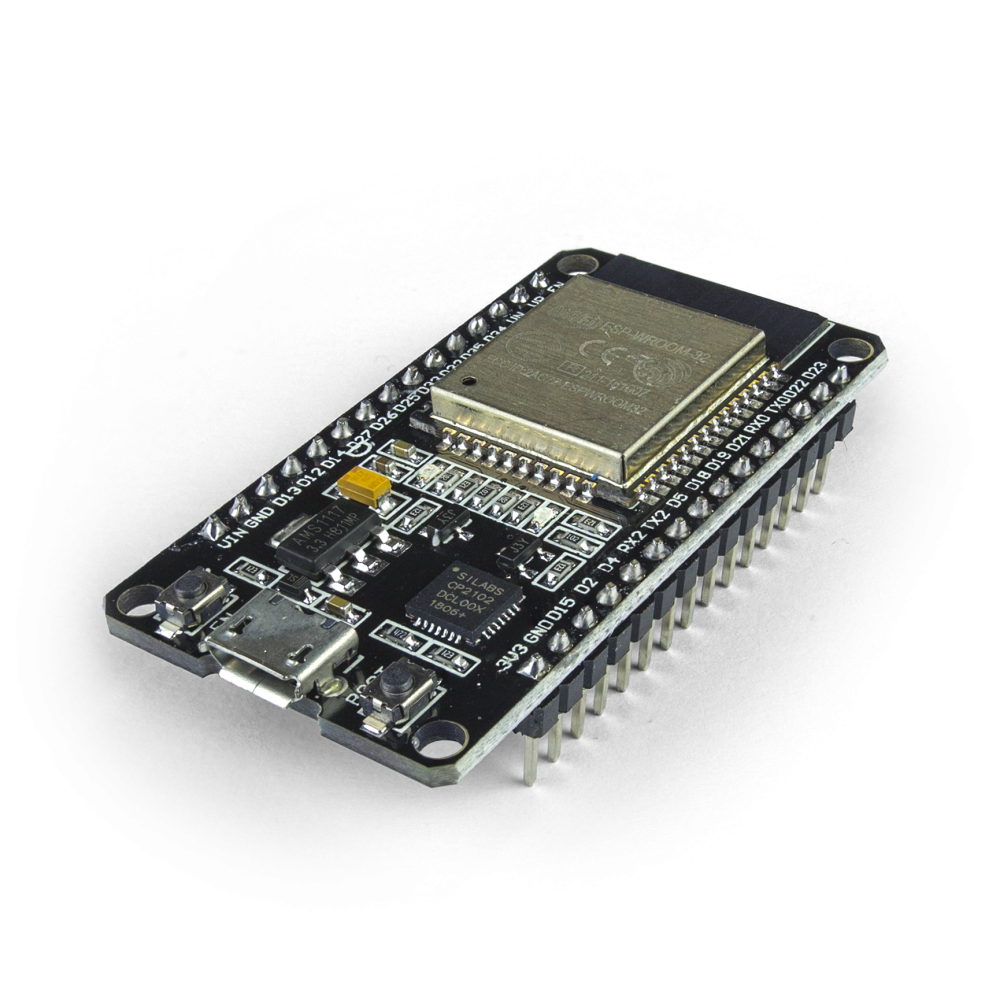
\includegraphics[width=8.5cm]{imagem/esp-wroom32.png} 
    \caption{Placa de prototipação com módulo ESP32}
    \label{fig:esp32-module}
\end{figure}

\subsection{Sensor HC-SR04}
HC-SR04 é um sensor ultrassônico de alcance que fornece a função de medição entre 2 cm a 400 cm sem contato \cite{electro}. Permite medir a distância do sensor até a superfície líquida, emitindo ondas sonoras, que são rebatidas na superfície e retorna para um receptor no equipamento \cite{tairaprototipagem}. É um componente amplamente disponível e são comercializadas unidades produzidas por diversos fabricantes diferentes.

\begin{figure}[ht]
    \centering
    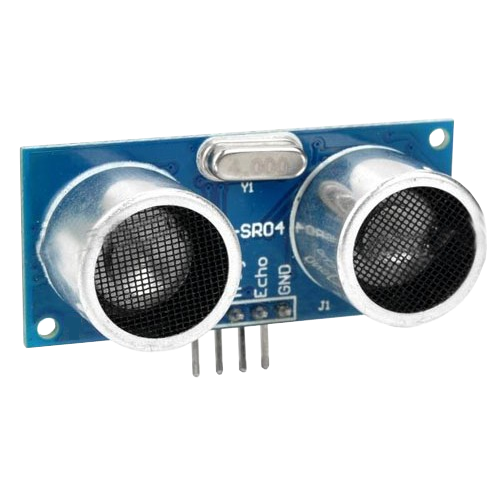
\includegraphics[width=6.5cm]{imagem/hc-sr04.png} 
    \caption{Sensor ultrassônico HC-SR04.}
    \label{fig:hc-sr04}
\end{figure}

\subsection{Mini Bomba D'água JT100}
Para as unidades de escoamento, foi utilizado uma mini bomba d’água que é usada submersa, já que seu sistema elétrico é vedado com nível de proteção IP68, além de trabalhar com tensões mais baixas entre 3V a 6V DC e com uma vazão entre 80 l/h a 120 l/h com eficiência e precisão, além de ser apropriada para prototipação com plataformas como Arduino \cite{usinainfo}. Este é também um componente amplamente disponível e são comercializadas unidades produzidas por diversos fabricantes diferentes.

\begin{figure}[ht]
    \centering
    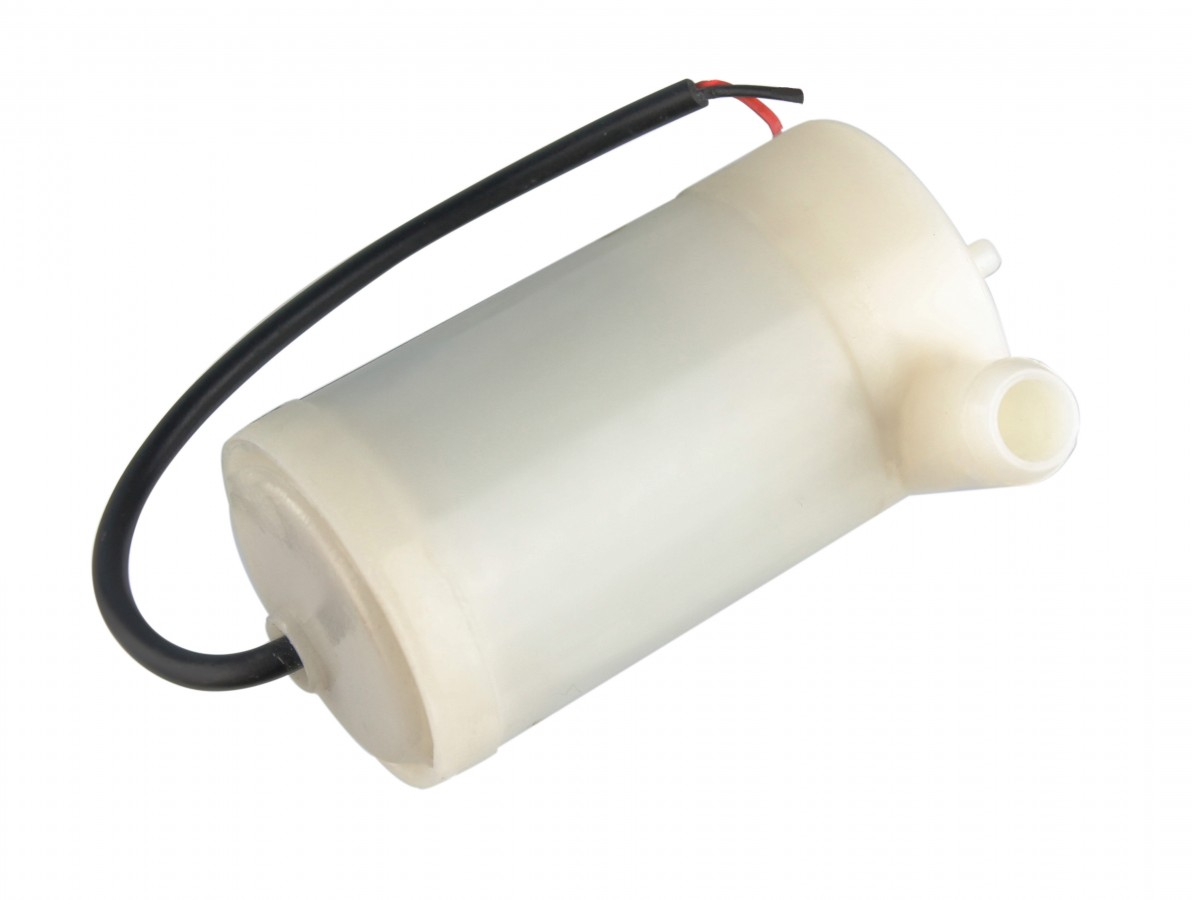
\includegraphics[width=6.5cm]{imagem/jt100.jpg} 
    \caption{Mini bomba d'água JT100.}
    \label{fig:mini-water-pump}
\end{figure}

\subsection{Transistor TIP41C NPN}
O TIP41C é um transistor NPN de alta potência podendo suportar uma tensão máxima de 100V e corrente máxima de 6A, e alta velocidade de chaveamento. Conforme informações do datasheet, sua ativação para correntes de coletor inferior a 0,01A é aproximadamente 630mV, sendo seu tempo de chaveamento para operações de baixa corrente de 3µs. \cite{utmel}.

\begin{figure}[ht]
    \centering
    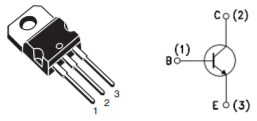
\includegraphics[width=6.8cm]{imagem/tip41c-w-schematic.png} 
    \caption{Transistor TIP41C NPN e seu diagrama interno}
    \label{fig:tip41c-npn}
\end{figure}

\subsection{Protocolo MQTT}
MQTT é um protocolo de transporte de mensagens do tipo \textit{publish/subscribe}. Projetado para ser leve, aberto, simples e fácil de implementar, é ideal para ser utilizado em soluções com ambientes limitados em hardware e software, para contextos de comunicação de máquina-a-máquina (M2M) e Internet das Coisas (IoT), onde memória e largura de banda são normalmente bastante limitados \cite{mqtt}.

Neste projeto, o protocolo MQTT é a base da comunicação entre as unidades, pois as leituras dos níveis dos contêineres são publicadas em um tópico específico, enquanto que o monitoramento, inscrito neste mesmo tópico, é capaz de obter e apresentar os dados para o operador, além de comandar o acionamento da unidade de escoamento conforme parâmetros pré-determinados. Da mesma forma, as unidades de escoamento, recebem informações sobre quando e o quanto escoar diretamente das unidades de monitoramento.

\subsection{Plataforma Node-RED}
Node-RED é uma plataforma low-code \cite{ibm-lowcode} para o desenvolvimento de aplicações baseadas em eventos \cite{nodered}, com uma interface baseada em \textit{nodes} (nós) que representam dispositivos e serviços, e através da interligação visual destes nodes é possível definir diversos tipos de fluxos que definem as funcionalidades das aplicações.

Com base na plataforma Node-RED, foi experimentado estender as funcionalidades propostas neste projeto, e como prova de conceito, foi implementado o monitoramento via navegador (\textit{browser}) com armazenamento dos dados das leituras dos sensores ultrassônicos em banco de dados relacional.

\subsection{RDBMS PostgreSQL}
PostgreSQL é um poderoso sistema de banco de dados relacional de objeto de código aberto com mais de 35 anos de desenvolvimento ativo que lhe rendeu uma forte reputação de confiabilidade, robustez de recursos e desempenho \cite{postgresql}.

Neste projeto, os dados lidos dos sensores ultrassônicos são gravados em um banco de dados PostgreSQL possibilitando a apresentação do histórico de variação dos níveis dos contêineres monitorados.

\clearpage

% ===== Trabalhos Correlatos =====
\newpage
\section{Trabalhos Correlatos}

\subsection{Taíra e Siqueira, 2018}

Daniel Taíra e Felipe Siqueira publicaram em 2018 um trabalho intitulado "PROTOTIPAGEM UTILIZANDO PLATAFORMA ARDUINO PARA SISTEMA DE CONTROLE DE NÍVEL" \cite{tairaprototipagem}. O projeto é desenvolvido de modo que os componentes (sensores) responsáveis pela medição, os componentes responsáveis pela movimentação do fluído (atuadores) e os módulos de controle, estão todos ligados em um sistema monolítico, capaz de fazer a movimentação do fluído de um tanque inferior para um tanque superior em um aparato onde todos os componentes, incluindo os tanques, sejam parte uma única peça.

\subsection{Matheus Gonçalves, 2019}

Matheus Gonçalves publicou em 2019 um trabalho intitulado "CONTROLE DE NÍVEL DE PLANTA DIDÁTICA USANDO CONTROLADOR LÓGICO PROGRAMÁVEL" \cite{gonccalves2019controle}. O projeto emprega o uso de um CLP didático em oposição à plataformas mais acessíveis como Arduíno ou ESP32. O propósito do projeto é controlar os níveis de fluídos entre três tanques, sendo que dois deles servem como reservatório de fluído para o tanque principal, que é o tanque monitorado medindo-se o nível através de um sensor ultrassônico HC-SR04. Os tanques reservatórios são mantidos dentro do mínimo e máximo através de sensores do tipo chave-boia. 

\subsection{Thalys Gadelha, 2020}

Thalys Gadelha publicou em 2020 um trabalho intitulado "SISTEMA PARA MONITORAMENTO DO NÍVEL DE ÁGUA EM RECIPIENTES DE ANIMAIS DOMÉSTICOS" \cite{gadelha2020sistema}. Trata-se de um projeto voltado para a manutenção de vasilhames para alimentação de animais domésticos. Utiliza ESP32 e sensores para determinar se o nível do conteúdo medido está abaixo de um nível considerado crítico, para então utilizar uma rede GSM para enviar notificações de SMS, além de um sinal sonoro (buzzer). Neste trabalho não há implementação de alimentação automática do conteúdo.

\subsection{Sumário da Correlação}

Embora os projetos mencionados tenham certas similaridades em relação a este projeto, todos eles apresentam a solução entre a medição, monitoramento e acionamento das bombas de escoamento ou alimentação em um bloco monolítico. Observa-se que os projetos citados estão muito mais focados na precisão da medição e do acionamento.

Este trabalho, por outro lado, preocupa-se mais com a infraestrutura e com a integração e comunicação entre os componentes, no sentido de que procura aplicar as características que distinguem a IoT, de modo a desenvolver uma plataforma para formação de uma rede de equipamentos capazes de medir e atuar de forma independente e com alto potencial de escalabilidade.


% ===== Desenvolvimento =====
\newpage
\section{Desenvolvimento}
Neste capítulo, serão apresentados os principais detalhes sobre o desenvolvimento do protótipo. Todos os códigos, diagramas esquemáticos e todos os detalhes para preparação da infraestrutura de software, estão disponíveis em um repositório no GitHub\footnote{URL: https://github.com/danielgoncalves/iot-ifsp-ctd-tcc. Acesso em: 25 nov. 2024.} dedicado a este trabalho de conclusão de curso.

\subsection{Unidades}
O sistema em questão consiste em três conjuntos principais, ou unidades distintas: 
\begin{itemize}
    \item Unidade de Monitoramento e Comando
    \item Unidade de Medição
    \item Unidade de Escoamento ou Alimentação
\end{itemize}

\subsection{Unidade de Monitoramento}
A Unidade de Monitoramento é composta por um módulo ESP32, um mostrador de cristal líquido de 16x2 (16 colunas por 2 linhas) e 3 botões de pressionamento. Como o nome sugere, sua função é receber os dados dos tópicos MQTT onde são publicados valores de leitura dos níveis pelas Unidades de Medição, além de possibilitar o ajuste do nível crítico de cada Unidade de Medição e de, opcionalmente, comandar manualmente o escoamento de uma determinada Unidade de Escoamento. Figuras \ref{fig:photo-monitoring-unit} e \ref{fig:schematic-monitoring-unit}.

\begin{figure}[h!]
    \centering
    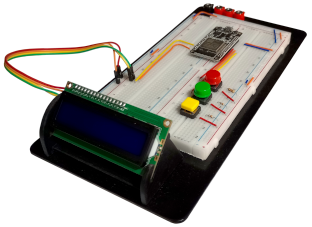
\includegraphics[width=7cm]{imagem/unidade-monitoramento.png}
    \caption{Protótipo da Unidade de Monitoramento}
    \label{fig:photo-monitoring-unit}
\end{figure}

\begin{figure}[h!]
    \centering
    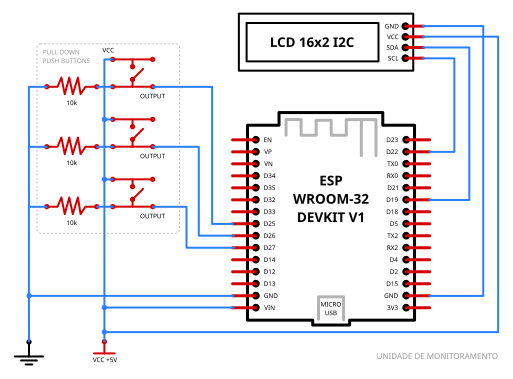
\includegraphics[width=9cm]{imagem/diagrama-unidade-monitoramento.png}
    \caption{Esquemático da Unidade de Monitoramento}
    \label{fig:schematic-monitoring-unit}
\end{figure}

\subsection{Unidade de Medição}
A Unidade de Medição é composta por um módulo ESP32 e um sensor ultrassônico HC-SR04. Pela proposta do trabalho, pode-se ter apenas uma Unidade de Medição ou várias. Para este trabalho foram desenvolvidas duas unidades para medição de dois conjuntos de contêineres. Sua função é medir o nível de um tanque ou contêiner e, atingido um determinado nível, que é configurado na própria unidade (ou através da Unidade de Monitoramento), é comandado escoamento de forma remota via MQTT. Figuras \ref{fig:photo-measure-unit} e \ref{fig:schematic-measure-unit}.

\begin{figure}[h!]
    \centering
    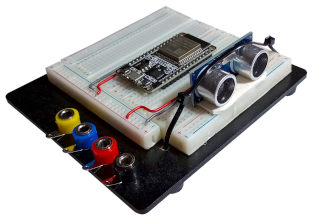
\includegraphics[width=7cm]{imagem/unidade-medicao.png}
    \caption{Protótipo da Unidade de Medição}
    \label{fig:photo-measure-unit}
\end{figure}

\begin{figure}[h!]
    \centering
    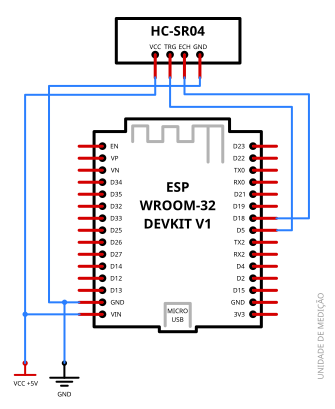
\includegraphics[width=7cm]{imagem/diagrama-unidade-medicao.png}
    \caption{Esquemático da Unidade de Medição}
    \label{fig:schematic-measure-unit}
\end{figure}

\subsection{Unidade de Escoamento}
A Unidade de Escoamento é composta por um módulo ESP32, um transistor TP41C NPN, e uma mini bomba d'água. O acionamento da bomba d'água é feito quando a unidade recebe uma mensagem MQTT indicando o tempo, em segundos, que a bomba deverá permanecer acionada. Figuras \ref{fig:photo-pump-unit} e \ref{fig:schematic-pump-unit}.

\begin{figure}[h!]
    \centering
    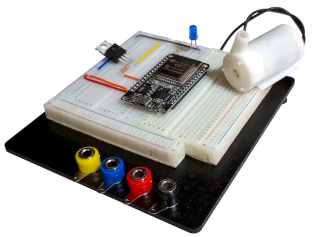
\includegraphics[width=7cm]{imagem/unidade-escoamento.png}
    \caption{Protótipo da Unidade de Escoamento}
    \label{fig:photo-pump-unit}
\end{figure}

\begin{figure}[h!]
    \centering
    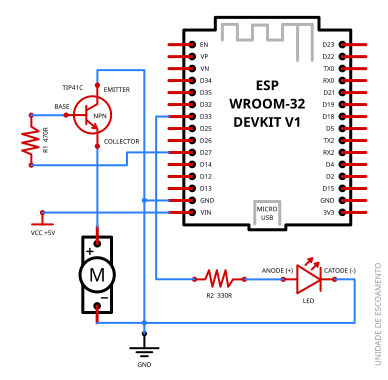
\includegraphics[width=0.5\linewidth]{diagrama-unidade-escoamento.png}
    \caption{Esquemático da Unidade de Escoamento}
    \label{fig:schematic-pump-unit}
\end{figure}

\subsection{Protótipo Montado}
A figura \ref{fig:mounted-aparatus} mostra as unidades protótipo, montadas próximas para facilitar o entendimento do aparato de hardware. Neste caso, a imagem mostra apenas uma unidade de medição e uma unidade de escoamento. Quando o contêiner que está sob a unidade de medição atinge o nível configurado, é comandado o escoamento para o contêiner ao lado.

\begin{figure}[h!]
    \centering
    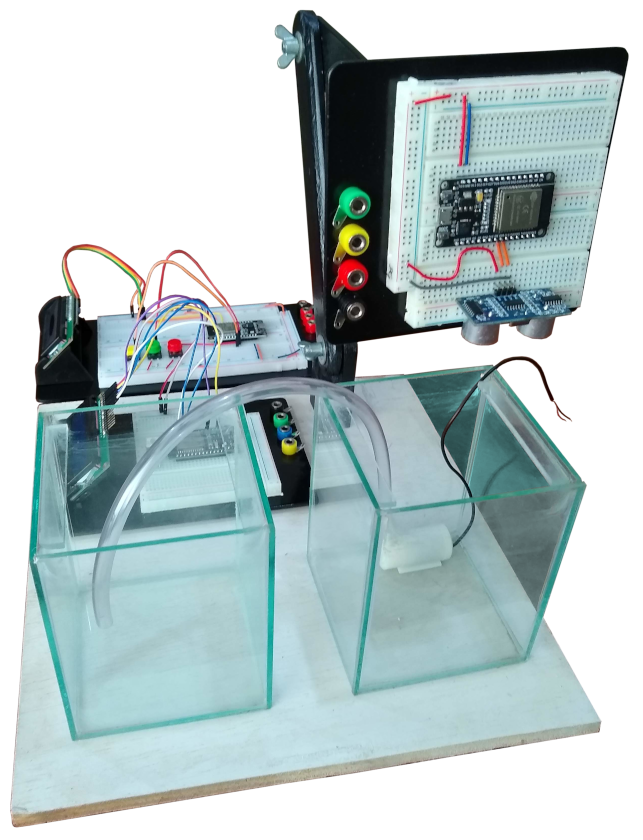
\includegraphics[width=11cm]{imagem/prototipo-montado-1.png}
    \caption{Unidades posicionadas próximas}
    \label{fig:mounted-aparatus}
\end{figure}

\subsection{Software}
Os códigos-fonte das unidades foram escritos em C++ (na verdade, abstrações em C++ sobre a linguagem Wiring\footnote{URL: https://wiring.org.co/. Acesso em: 31 ago. 2023.}) através do ambiente integrado de desenvolvimento (IDE) para Arduino\footnote{URL: https://www.arduino.cc/en/software}. 

\subsection{Infraestrutura para Comunicação}
A comunicação entre as unidades ocorre através do protocolo MQTT. Para isso é necessário um software servidor que implemente o protocolo MQTT. Neste projeto utilizamos a implementação do Eclipse Mosquitto. 

\subsection{Infraestrutura para Logging e Monitoramento}
As leituras feitas pelas unidades de medição ficam registradas em um banco de dados relacional (RBDMS) PostgreSQL. O registro das leituras é feito por um fluxo específico, através da plataforma Node-RED, onde os dados que chegam no tópico "p/container/level"\space são registrados em uma tabela específica.
Também através da plataforma Node-RED, foram implementados fluxos para visualização dos níveis dos contêineres em um painel de instrumentação (\textit{dashboard}) que pode ser visualizado através de um navegador de internet (\textit{web browser}, figura \ref{fig:dashboard-node-red}). O fluxo Node-RED utilizado está disponível no repositório do projeto em \url{https://github.com/danielgoncalves/iot-ifsp-ctd-tcc/blob/main/Infra/Node-RED/flow.json}, figura \ref{fig:node-red-ui}.

\begin{figure}[h!]
    \centering
    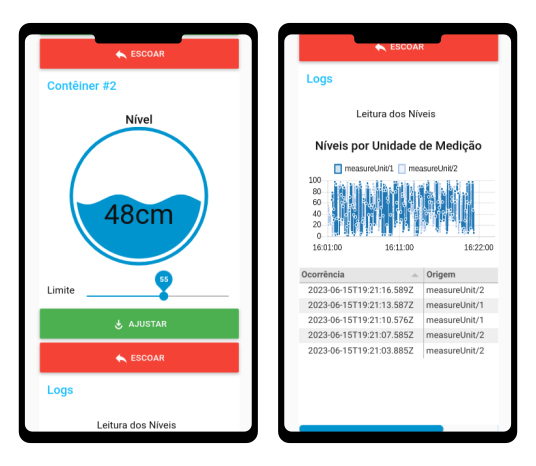
\includegraphics[width=12cm]{imagem/dashboard-mobile.png}
    \caption{Dashboard implementado via Node-RED}
    \label{fig:dashboard-node-red}
\end{figure}

\begin{figure}[h!]
    \centering
    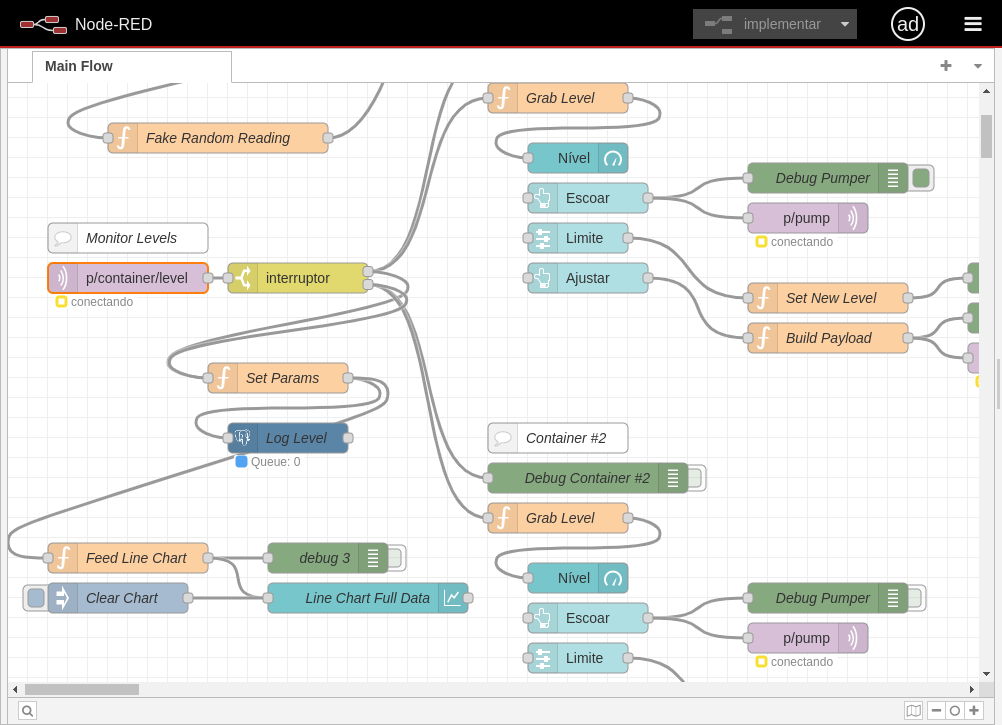
\includegraphics[width=0.5\linewidth]{imagem/node-red-ui.png}
    \caption{Interface do Node-RED com o fluxo deste projeto}
    \label{fig:node-red-ui}
\end{figure}

\subsection{Implementação da Infraestrutura}
Para disponibilizar os serviços de software citados nos tópicos anteriores, optou-se por utilizar virtualização baseada em \textit{containers} Docker\footnote{URL: https://docs.docker.com/}. Por serem relativamente leves, é possível executar todos os serviços necessários em um único hospedeiro baseado em Linux, e testar toda a implementação do projeto em rede local.

Porém, essa mesma infraestrutura pode ser disponibilizada em uma instância AWS EC2\footnote{URL: https://aws.amazon.com/pt/ec2/} e ter os serviços disponibilizados de forma ampla via internet.

\clearpage



% ===== Conclusão =====
\newpage
\section{Conclusão}
O sistema proposto oferece uma solução robusta e escalável para o monitoramento e controle de nível de fluído em contêineres. A integração de sensores ultrassônicos, microcontroladores ESP32 e protocolo MQTT permite uma comunicação eficiente entre os dispositivos, enquanto a infraestrutura de serviços oferece recursos avançados de monitoramento e registro (\textit{logging}).

Partindo de um protótipo minimamente funcional, há um enorme espaço para implementação de melhorias, desde os detalhes relacionados à precisão da leitura dos níveis dos contêineres, incluindo testes de interferência no sensor ultrassônico utilizado, até a implementação de balanceadores de carga e escalabilidade automatizada de serviços que considere o aumento da demanda de dispositivos de medição adicionados ao conjunto.

%==============================BIBLIOGRAFIA=================================
\newpage
\renewcommand{\bibname}{REFERÊNCIAS}
\bibliography{bibliography}

\end{document}
